\newpage
\subsection{Modelo de información - Diagrama de comunicación}
El modelo de información ayuda a entender e implementar el comportamiento del sistema \textbf{QuickContentMedia}.

Los diagramas fueron elaborados utilizando la herramienta {Visual Paradigm}. La imagen \ref{DiagComu} muestra el diagrama de comunicación DC-001 correspondiente al caso de uso CU-001 Acceder al portal.

%%%%%%%%%%%%%%%%%%%%%%%%%%%Configuracion Tabla

\begin{figure}[H]
    \centering
    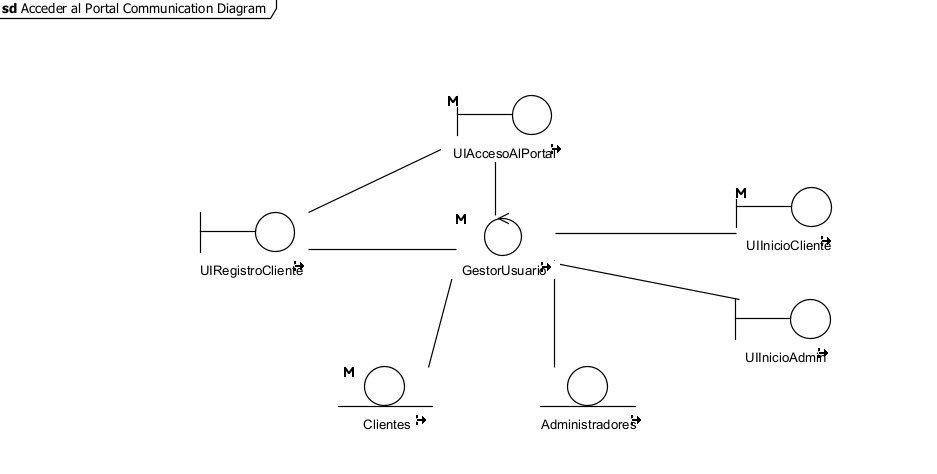
\includegraphics[width=0.95\linewidth]{Media/3_Analisis/3_ModeloDeRequisitos/DC-001.png}
    \caption{Diagrama de comunicación DC-001}
    \label{DiagComu}
\end{figure}

%%%%%%%%%%%%%%%%% FIN tabla
\textbf{Archivo:} {Diagramas de Comunicación} \\
\textbf{Link de acceso:} \linkDiagramaComunicacion \\

\textbf{Pasos de ejecución:}
\begin{itemize}
    \item Ingresar al repositorio en GitHub usando el link proporcionado y descargar el archivo QCM.vpp
    \item Abrir el archivo descargado en la herramienta Visual Paradigm.
    \item En la pestaña Diagram Navigator abrir UML Diagrams
    \item Abrir Communication Diagram y seleccionar el diagrama de comunicación que se desee visualizar.
\end{itemize}

\textbf{Documento:} {Diccionario del diagrama de Comunicación} \\
\textbf{Link de acceso:} \linkDiccionarioComunicacion \\

